% Source: graduate-coursework/Research/Papers/drafts/click_supervision_prelabeling/Radar_Annotation_PreLabeling_ClickSupervision.tex
% Description: Overview of the proposed pre-labelling and click-to-annotate pipeline for marine radar PPI images.

\documentclass[border=4pt]{standalone}
\usepackage{amsmath,amssymb}
\usepackage{graphicx}
\usepackage{tikz}
\usetikzlibrary{arrows.meta,positioning}

\begin{document}
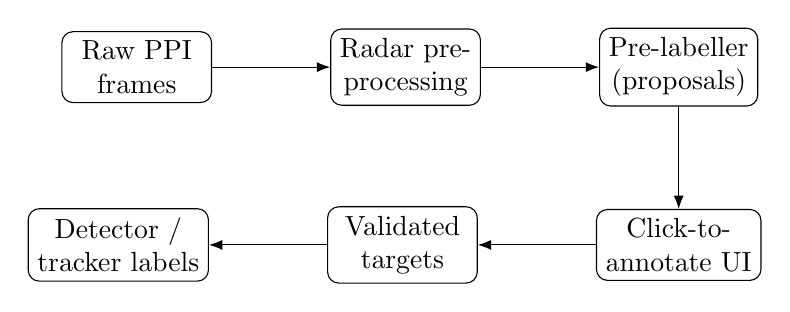
\begin{tikzpicture}[
        node distance=1.5cm,
        >=Latex,
        process/.style={rectangle, rounded corners, draw, align=center, minimum width=1.9cm, minimum height=0.9cm}
    ]
        \node[process] (raw) {Raw PPI\\frames};
        \node[process, right=1.5cm of raw] (pre) {Radar pre-\\processing};
        \node[process, right=1.5cm of pre] (pl) {Pre-labeller\\(proposals)};
        \node[process, below=1.3cm of pl] (ui) {Click-to-\\annotate UI};
        \node[process, left=1.5cm of ui] (labels) {Validated\\targets};
        \node[process, left=1.5cm of labels] (export) {Detector /\\tracker labels};

        \draw[->] (raw) -- (pre);
        \draw[->] (pre) -- (pl);
        \draw[->] (pl) -- (ui);
        \draw[->] (ui) -- (labels);
        \draw[->] (labels) -- (export);
    \end{tikzpicture}
\end{document}
